\documentclass{article}
\usepackage{graphicx}
\usepackage[margin=1.5cm]{geometry}
\usepackage{amsmath}

\begin{document}

\title{Tuesday Reading Assessment: Unit 3, Magnetic Forces and Fields}
\author{Prof. Jordan C. Hanson}

\maketitle

\section{Memory Bank}

\begin{itemize}
\item $\hat{i} \times \hat{j} = \hat{k}$, $\hat{j} \times \hat{k} = \hat{i}$, $\hat{k} \times \hat{i} = \hat{j}$ ... The direction of the \textit{cross-product} follows this pattern.  Reversing the order of any two vectors introduces a minus sign.
\item $\hat{i} \times \hat{i} = 0$, $\hat{j} \times \hat{j} = 0$, $\hat{k} \times \hat{k} = 0$ ... The \textit{cross-product} is zero when both vectors are parallel.
\item $|\vec{a} \times \vec{b}| = |\vec{a}||\vec{b}|\sin\theta$ ... The magnitude of the cross-product of two vectors $\vec{a}$ and $\vec{b}$, given the angle $\theta$ between them.
\item $\vec{F} = i\vec{L} \times \vec{B}$ ... The Lorentz force, by a magnetic field $\vec{B}$ on a \textit{current} $i$ of length and direction $\vec{L}$.
\end{itemize}

\section{The Cross-Product}

\begin{enumerate}
\item Let $\vec{a} = 4\hat{i}$, and $\vec{b} = 4\hat{j}$.  (a) Calculate $\vec{a} \times \vec{b}$. (b) What are the magnitude and direction of the result? \\ \vspace{0.5cm}
\item Let $\vec{a} = 2\hat{i} + 2\hat{j}$, and $\vec{b} = -2\hat{i} - 2\hat{j}$.  (a) Calculate $\vec{a} \times \vec{b}$. (b) What are the magnitude and direction of the result? \\ \vspace{0.5cm}
\item What is the angle between the two vectors in the previous problem?
\end{enumerate}

\section{Magnetic Force on a Wire}

\begin{enumerate}
\item Consider Fig. \ref{fig:1}, in which a current passes through a \textit{magnetic field} generated by a permanent magnet.  Notice in the Memory Bank the formula for the force on the conductor carrying the current.  (a) If the amount of wire in the magnetic field is $L = 10$ cm, the magnetic field is $B = 10^{-1}$ Tesla, the voltage is $V = 24$ Volts, and the effective resistance in the wire is $R = 2\Omega$, what is the force upwards on the wire? (b)  If the wire was attached to a scale, and the scale has a mass of $m = 24$ grams on it, what would the scale read if we turn on this current in this magnetic field?  (\textit{Hint: it won't say 24 grams}).
\end{enumerate}

\begin{figure}
\centering
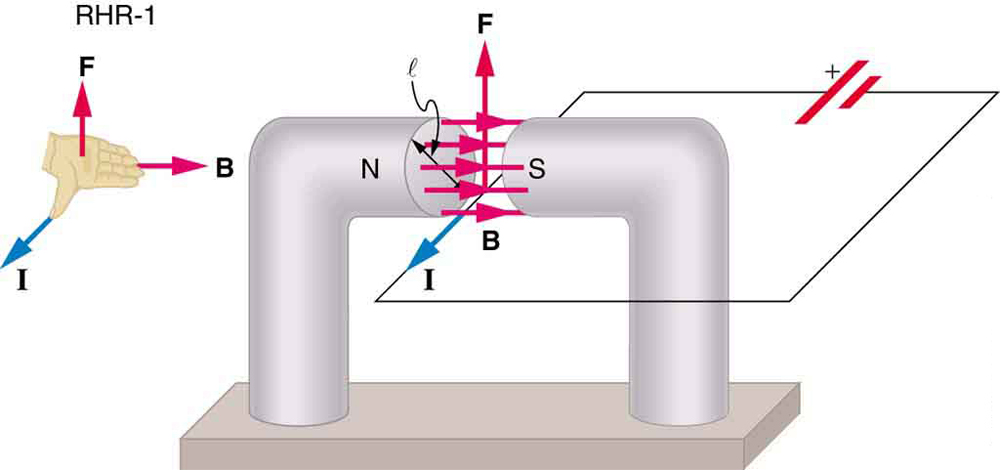
\includegraphics[width=0.5\textwidth]{figures/force.jpeg}
\caption{\label{fig:1} A permanent magnet creates a magnetic field to the \textit{left}, while a voltage pushes a current \textit{out of the page}.  The force is measured to occur in the \textit{upward direction}.}
\end{figure}

\end{document}
